\documentclass{beamer}

\usepackage[utf8]{inputenc}
\usepackage{default}
\usepackage[italian]{babel}
\usepackage{color}
%\usetheme{Picx}
\colorlet{Green}{green!40!black}


\title{EigenNet}
\subtitle{\textsc{\large Reti wireless mesh con Linux}}
%\author{Gioacchino Mazzurco}
%\date{27 ottobre 2012}
%\institute{eigenLab}
\date{}
\hypersetup{pdfauthor={Gioacchino Mazzurco, Ilario Gelmetti},pdfsubject={EigenNet - The open wireless community in Pisa.},pdfkeywords={mesh, wireless, eigennet, italy, pisa, eigenlab, community, ninux, ubiquiti, awmn, guifi, open, openwrt, batman, batman-adv},pdftitle={EigenNet - Reti wireless mesh con Linux.}}

\begin{document}
\title{\vspace{30pt}}
\begin{frame}
\titlepage   \vspace{-2.3cm}
\begin{center}
{\bf Gioacchino Mazzurco} \vspace{0.3cm}

\small 27 ottobre 2012\end{center} \vspace{0.5cm}
\flushleft \hspace{2.8cm} {\url{eigenlab.org}}\\ \vspace{1cm} 
\hspace{2.8cm} {\url{wiki.ninux.org}}


\begin{picture}(0,0)(-200,40)
\put(-118,217){
\includegraphics[scale=4]{images/eigennet.png}}
\put(-220,80){
\includegraphics[width=0.3\textwidth]{images/eigenlab-small.png}}
\put(-220,50){
\includegraphics[width=0.3\textwidth]{images/ninux-indicizzato.png}}
\put(40,70){
\includegraphics[scale=0.25]{images/linuxday-small.png}}
\end{picture}

 \end{frame}
\title{\textsc{EigenNet} - reti wireless mesh con Linux}
\author{Gioacchino Mazzurco}
\date{27 ottobre 2012}
\institute{eigenLab}
\section{Introduzione}

\subsection{Cos'è EigenNet}
\logo{
\includegraphics[width=0.1\paperwidth]{images/eigenlab-small.png}}
\begin{frame}\frametitle{Cos'è EigenNet}
\textbf{\color{Green}EigenNet} è una \emph{rete comunitaria} principalmente wireless,\\ una \emph{\color{green}wireless community network}.
\vspace{5pt}

\hspace{1cm}\emph{Rete comunitaria: rete di telecomunicazione costruita da\\\hspace{3.9cm} una o più comunità di persone.}

\vspace{15pt}\pause


Da non confondere con la ``Wireless del Comune''.
\begin{picture}(0,0)(0,0)
\put(-5,-10){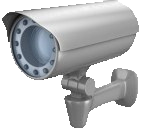
\includegraphics[scale=0.2]{images/telesorveglianza.png}}
\end{picture}
\end{frame}

\setbeamercovered{dynamic}

\subsection{Ma che differenza c'è da quella del Comune?}
\begin{frame}\frametitle{Ma che differenza c'è da quella del Comune?}
\begin{itemize}
 \item \textbf{\color{blue}Community Based}: Le politiche di sviluppo sono decise dai partecipanti in modo paritario.
\pause
 \item \textbf{\color{blue}Open}: 
  \begin{itemize}
  \item nessuna autenticazione richiesta (decisione delegata ai singoli gateway) e nessuna discriminazione all'accesso.
  \item Utilizzo di software libero (OpenWrt, Gentoo, BATMAN-adv, $\cdots$).
  \item Nessuna crittografia sul segnale radio, come nella Wireless del Comune. Sicurezza delegata a livello applicazione.
  \end{itemize}
\pause
\item \textbf{\color{blue}Contro la censura}: All'interno della rete non c'è censura (già presenti link internazionali che bypassano i filtri nazionali), verso internet si può scegliere tra vari gateway su vari ISP (assenza di censura = arma per la democrazia).


\end{itemize}
\end{frame}
\begin{frame}\frametitle{Ma che differenza c'è da quella del Comune? - 2}
\begin{itemize}
 
 \item \textbf{\color{blue}Decentralizzata}: I partecipanti sono proprietari solamente di una piccola parte dell’infrastruttura, non c’è un'unica entità proprietaria della rete.
\pause
 \item \textbf{\color{blue}Resiliente}: Il routing è dinamico, se una antenna si spegne la rete si adatta, non crolla.

\pause
 \item \textbf{\color{blue}Resistente}: Nessun bisogno di server né di internet (un terremoto? un Mubarak? \emph{Garantisce la connettività locale}), serve solo poca corrente elettrica (pannelli solari?).
\end{itemize}
\end{frame}


\subsection{Praticamente?}
\begin{frame}\frametitle{Praticamente?}
      \textbf{\color{blue}Cosa costituisce una rete comunitaria?}
      \begin{itemize}
	\item persone attive,
	\item motivazioni,
	\item antenne,
	\item protocollo di routing,
	\item firmware,
	\item configurazione,
	\item collegamenti wireless e via cavo,
	\item utenti non attivi,
	\item servizi
	\begin{itemize}
	  \item ADSL condiviso o acquisto di banda all'ingrosso,
	  \item voip, siti, chat, p2p, streaming video e audio,
	  \item $\cdots$
	\end{itemize}
      \end{itemize}
\begin{picture}(0,0)(0,0)
\end{picture}
\end{frame}

 

\begin{frame}\frametitle{Praticamente?}
      Cosa costituisce una rete comunitaria?
      \begin{itemize}
	\item \textbf{\color{blue}persone attive},
	\item motivazioni,
	\item antenne,
	\item protocollo di routing,
	\item firmware,
	\item configurazione,
	\item collegamenti wireless e via cavo,
	\item utenti non attivi,
	\item servizi
	\begin{itemize}
	  \item ADSL condiviso o acquisto di banda all'ingrosso,
	  \item voip, siti, chat, p2p, streaming video e audio,
	  \item $\cdots$
	\end{itemize}
      \end{itemize}
\begin{picture}(0,0)(0,0)
\put(200,60){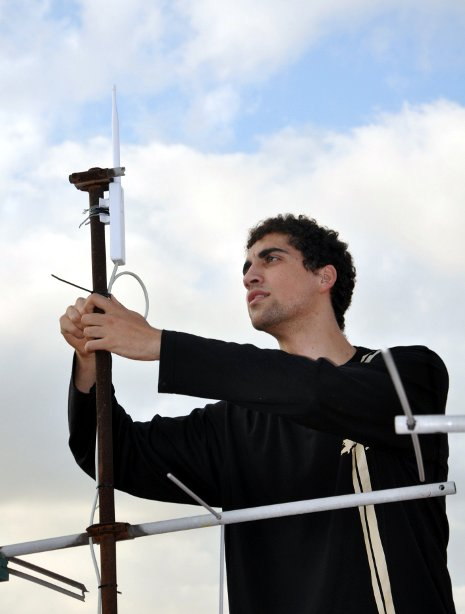
\includegraphics[scale=0.2]{images/gioacchino-small.jpg}}
\end{picture}
\end{frame}


\begin{frame}\frametitle{Praticamente?}
      Cosa costituisce una rete comunitaria?
      \begin{itemize}
	\item persone attive,
	\item \textbf{\color{red}motivazioni},
	\item antenne,
	\item protocollo di routing,
	\item firmware,
	\item configurazione,
	\item collegamenti wireless e via cavo,
	\item utenti non attivi,
	\item servizi
	\begin{itemize}
	  \item ADSL condiviso o acquisto di banda all'ingrosso,
	  \item voip, siti, chat, p2p, streaming video e audio,
	  \item $\cdots$
	\end{itemize}
      \end{itemize}
\begin{picture}(0,0)(0,0)
\put(200,60){
\includegraphics[width=0.4\textwidth]{images/mignoloprof-indicizzata.png}}
\end{picture}
\end{frame}


\begin{frame}\frametitle{Praticamente?}
      Cosa costituisce una rete comunitaria?
      \begin{itemize}
	\item persone attive,
	\item motivazioni,
	\item \textbf{\color{blue}antenne},
	\item protocollo di routing,
	\item firmware,
	\item configurazione,
	\item collegamenti wireless e via cavo,
	\item utenti non attivi,
	\item servizi
	\begin{itemize}
	  \item ADSL condiviso o acquisto di banda all'ingrosso,
	  \item voip, siti, chat, p2p, streaming video e audio,
	  \item $\cdots$
	\end{itemize}
      \end{itemize}
\begin{picture}(0,0)(0,0)
\put(250,40){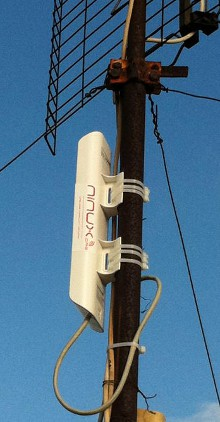
\includegraphics[scale=0.4]{images/antenne-small-small.jpg}}
\put(180,60){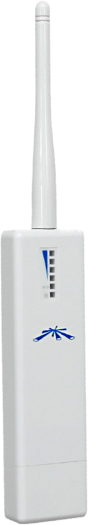
\includegraphics[scale=0.25]{images/UbiquitiPicoStationM2HP-small.png}}
\end{picture}
\end{frame}





\begin{frame}\frametitle{Praticamente?}
      Cosa costituisce una rete comunitaria?
      \begin{itemize}
	\item persone attive,
	\item motivazioni,
	\item antenne,
	\item \textbf{\color{blue}protocollo di routing},
	\item firmware,
	\item configurazione,
	\item collegamenti wireless e via cavo,
	\item utenti non attivi,
	\item servizi
	\begin{itemize}
	  \item ADSL condiviso o acquisto di banda all'ingrosso,
	  \item voip, siti, chat, p2p, streaming video e audio,
	  \item $\cdots$
	\end{itemize}
      \end{itemize}
\begin{picture}(0,0)(0,0)
\put(200,120){
\includegraphics[width=0.4\textwidth]{images/batman-adv.png}}
\end{picture}
\end{frame}


\begin{frame}\frametitle{Praticamente?}
      Cosa costituisce una rete comunitaria?
      \begin{itemize}
	\item persone attive,
	\item motivazioni,
	\item antenne,
	\item protocollo di routing,
	\item \textbf{\color{blue}firmware},
	\item configurazione,
	\item collegamenti wireless e via cavo,
	\item utenti non attivi,
	\item servizi
	\begin{itemize}
	  \item ADSL condiviso o acquisto di banda all'ingrosso,
	  \item voip, siti, chat, p2p, streaming video e audio,
	  \item $\cdots$
	\end{itemize}
      \end{itemize}
\begin{picture}(0,0)(0,0)
\put(200,105){
\includegraphics[scale=0.3]{images/openwrt.png}}
\end{picture}
\end{frame}

\begin{frame}\frametitle{Praticamente?}
      Cosa costituisce una rete comunitaria?
      \begin{itemize}
	\item persone attive,
	\item motivazioni,
	\item antenne,
	\item protocollo di routing,
	\item firmware,
	\item \textbf{\color{blue}configurazione},
	\item collegamenti wireless e via cavo,
	\item utenti non attivi,
	\item servizi
	\begin{itemize}
	  \item ADSL condiviso o acquisto di banda all'ingrosso,
	  \item voip, siti, chat, p2p, streaming video e audio,
	  \item $\cdots$
	\end{itemize}
      \end{itemize}
\begin{picture}(0,0)(0,0)
\put(200,100){
\includegraphics[width=0.4\textwidth]{images/eigennet.png}}
\end{picture}
\end{frame}

\begin{frame}\frametitle{Praticamente?}
      Cosa costituisce una rete comunitaria?
      \begin{itemize}
	\item persone attive,
	\item motivazioni,
	\item antenne,
	\item protocollo di routing,
	\item firmware,
	\item configurazione,
	\item \textbf{\color{blue}collegamenti wireless e via cavo},
	\item utenti non attivi,
	\item servizi
	\begin{itemize}
	  \item ADSL condiviso o acquisto di banda all'ingrosso,
	  \item voip, siti, chat, p2p, streaming video e audio,
	  \item $\cdots$
	\end{itemize}
      \end{itemize}
\begin{picture}(0,0)(0,0)
\put(220,53){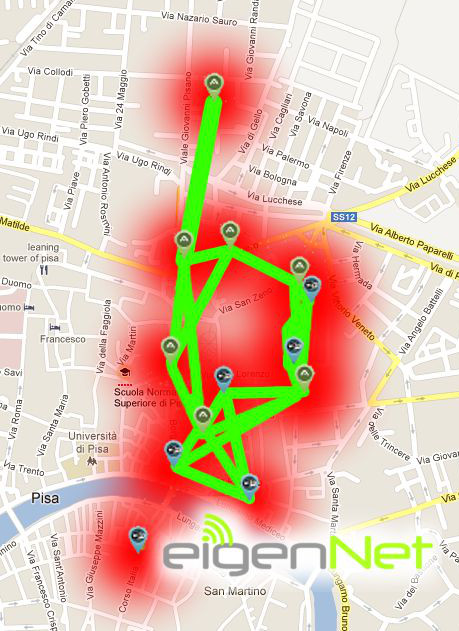
\includegraphics[width=0.36\textwidth]{images/mappa.jpg}}
\end{picture}
\end{frame}

\begin{frame}\frametitle{Praticamente?}
      Cosa costituisce una rete comunitaria?
      \begin{itemize}
	\item persone attive,
	\item motivazioni,
	\item antenne,
	\item protocollo di routing,
	\item firmware,
	\item configurazione,
	\item collegamenti wireless e via cavo,
	\item \textbf{\color{blue}utenti non attivi},
	\item servizi
	\begin{itemize}
	  \item ADSL condiviso o acquisto di banda all'ingrosso,
	  \item voip, siti, chat, p2p, streaming video e audio,
	  \item $\cdots$
	\end{itemize}
      \end{itemize}
\begin{picture}(0,0)(0,0)
\put(200,60){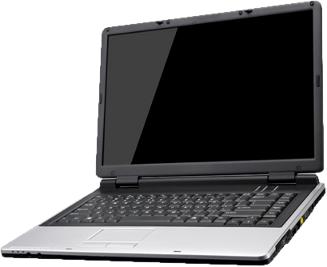
\includegraphics[width=0.36\textwidth]{images/portatile-small.png}}
\put(160,100){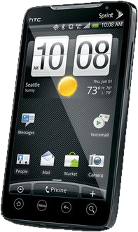
\includegraphics[width=0.1\textwidth]{images/htc-evo-small.png}}
\end{picture}
\end{frame}

\begin{frame}\frametitle{Praticamente?}
      Cosa costituisce una rete comunitaria?
      \begin{itemize}
	\item persone attive,
	\item motivazioni,
	\item antenne,
	\item protocollo di routing,
	\item firmware,
	\item configurazione,
	\item collegamenti wireless e via cavo,
	\item utenti non attivi,
	\item servizi
	\begin{itemize}
	  \item \textbf{\color{blue}ADSL condiviso e acquisto di banda all'ingrosso},
	  \item voip, siti, chat, p2p, streaming video e audio,
	  \item $\cdots$
	\end{itemize}
      \end{itemize}
\begin{picture}(0,0)(0,0)
\put(200,60){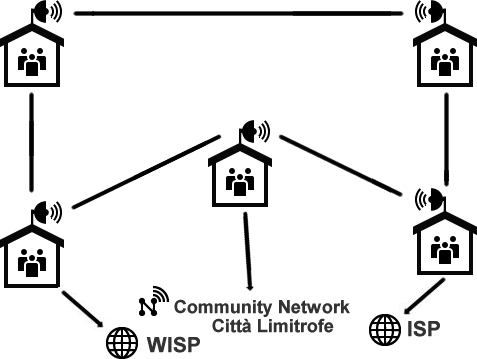
\includegraphics[width=0.4\textwidth]{images/digitaldivide-ridotto.png}}
\end{picture}
\end{frame}

\begin{frame}\frametitle{Praticamente?}
      Cosa costituisce una rete comunitaria?
      \begin{itemize}
	\item persone attive,
	\item motivazioni,
	\item antenne,
	\item protocollo di routing,
	\item firmware,
	\item configurazione,
	\item collegamenti wireless e via cavo,
	\item utenti non attivi,
	\item servizi
	\begin{itemize}
	  \item ADSL condiviso o acquisto di banda all'ingrosso,
	  \item \textbf{\color{blue}voip, siti, chat, streaming video e audio},
	  \item $\cdots$
	\end{itemize}
      \end{itemize}
\begin{picture}(0,0)(0,0)
\put(170,160){
\includegraphics[width=0.15\textwidth]{images/owncloud.png}}
\put(170,110){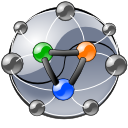
\includegraphics[width=0.1\textwidth]{images/retroshare.png}}\put(163,100){\footnotesize RetroShare}
\put(230,55){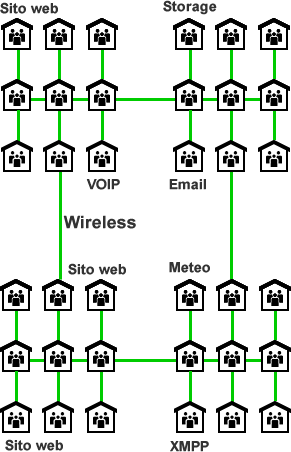
\includegraphics[width=0.32\textwidth]{images/servizi-interni-girata.png}}
\end{picture}
\end{frame}

\begin{frame}\frametitle{Praticamente?}
      Cosa costituisce una rete comunitaria?
      \begin{itemize}
	\item persone attive,
	\item motivazioni,
	\item antenne,
	\item protocollo di routing,
	\item firmware,
	\item configurazione,
	\item collegamenti wireless e via cavo,
	\item utenti non attivi,
	\item servizi
	\begin{itemize}
	  \item ADSL condiviso o acquisto di banda all'ingrosso,
	  \item voip, siti, chat, p2p, streaming video e audio,
	  \item \textbf{\color{blue}\Huge...}
	\end{itemize}
      \end{itemize}
\begin{picture}(0,0)(0,0)
\put(200,60){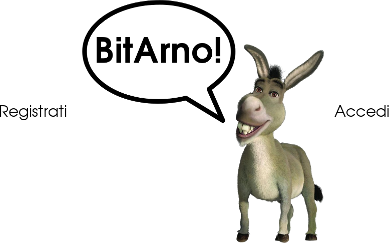
\includegraphics[width=0.4\textwidth]{images/bitarno-ritagliata-small.png}}
\end{picture}
\end{frame}

\section{La struttura}

\subsection{Infrastruttura fisica}
\begin{frame}\frametitle{Infrastruttura fisica}
\begin{itemize}
 \item \textbf{\color{blue}Nodi con antenne omnidirezionali}
\begin{itemize}
 \item circa 100 euro di costo.
 \item Buona affidabilità.
 \item Soffre il rumore da parte di altre antenne.
 \item Prestazioni basse (54 mbps).
 \item Collegamenti multipli ma minori di 1 km.
 \item Facile montaggio.
\end{itemize}
 \item Nodi con antenne direzionali
 \item Cavo
 \item Fibra ottica
\end{itemize}
\begin{picture}(0,0)(0,0)
\put(240,30){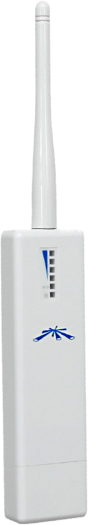
\includegraphics[scale=0.25]{images/UbiquitiPicoStationM2HP-small.png}}
\end{picture}
\end{frame}

\begin{frame}\frametitle{Infrastruttura fisica}
\begin{itemize}
 \item Nodi con antenne omnidirezionali
 \item \textbf{\color{blue}Nodi con antenne direzionali}
\begin{itemize}
 \item dai 200 euro di costo.
 \item Minor sensibilità al rumore.
 \item Prestazioni medie (150 mbps).
 \item Collegamento singolo (o quasi) fino a 50 km.
 \item Complicazioni nel montaggio\\(puntamento a volte difficoltoso).
\end{itemize}
 \item Cavo
 \item Fibra ottica
\end{itemize}
\begin{picture}(0,0)(0,0)
\put(250,30){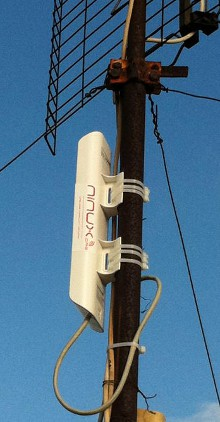
\includegraphics[scale=0.35]{images/antenne-small-small.jpg}}
\put(140,-35){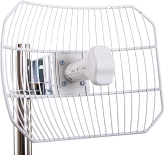
\includegraphics[scale=0.4]{images/airgrid-small.png}}
\end{picture}
\end{frame}

\logo{}

{\setbeamertemplate{navigation symbols}{}
\begin{frame}\frametitle{Infrastruttura fisica}
\begin{itemize}
 \item Nodi con antenne omnidirezionali
 \item Nodi con antenne direzionali
 \item \textbf{\color{blue}Cavo}
\begin{itemize}
 \item circa 0.50 euro al metro.
 \item Rare interferenze.
 \item Rare rotture.
 \item Prestazioni buone (1 gbps).
 \item Collegamenti corti (100 m). 
 \item Non sempre possibile.
\end{itemize}
 \item Fibra ottica
\end{itemize}
\begin{picture}(0,0)(0,0)
\put(235,104.5){\reflectbox{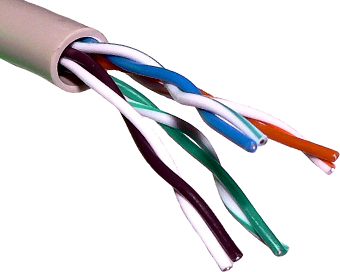
\includegraphics[scale=0.3]{images/utp_cable-small.png}}}
\put(235,30){\scalebox{-1}[-1]{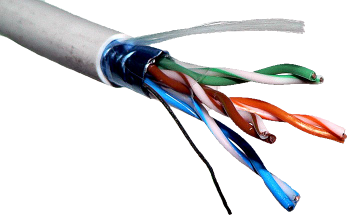
\includegraphics[scale=0.3]{images/ftp_cable-small.png}}}
\end{picture}
\end{frame}}
\logo{
\includegraphics[width=0.1\paperwidth]{images/eigenlab-small.png}}


\begin{frame}\frametitle{Infrastruttura fisica}
\begin{itemize}
 \item Nodi con antenne omnidirezionali
 \item Nodi con antenne direzionali
 \item Cavo
 \item \textbf{\color{blue}Fibra ottica}
\begin{itemize}
 \item circa 5 euro al metro.
 \item Costo strumentazione elevato.
 \item Interferenze assenti.
 \item Fragile.
 \item Prestazioni ottime (10 gbps).
 \item Collegamenti lunghi (molti km).
 \item Non sempre possibile.
\end{itemize}
\end{itemize}
\end{frame}


\subsection{Routing}
\begin{frame}\frametitle{Routing}
\begin{columns}
\column{0.5\linewidth}La rete è a maglie: \textbf{\color{blue} molti percorsi possibili}.\\\pause
Ogni nodo si annuncia come tale tramite messaggi HELLO.\\
In base al numero di HELLO ricevuti ogni nodo stabilisce la qualità del link e decide come instradare il traffico che lo attraversa.
\column{0.6\linewidth}\begin{figure}{\centering{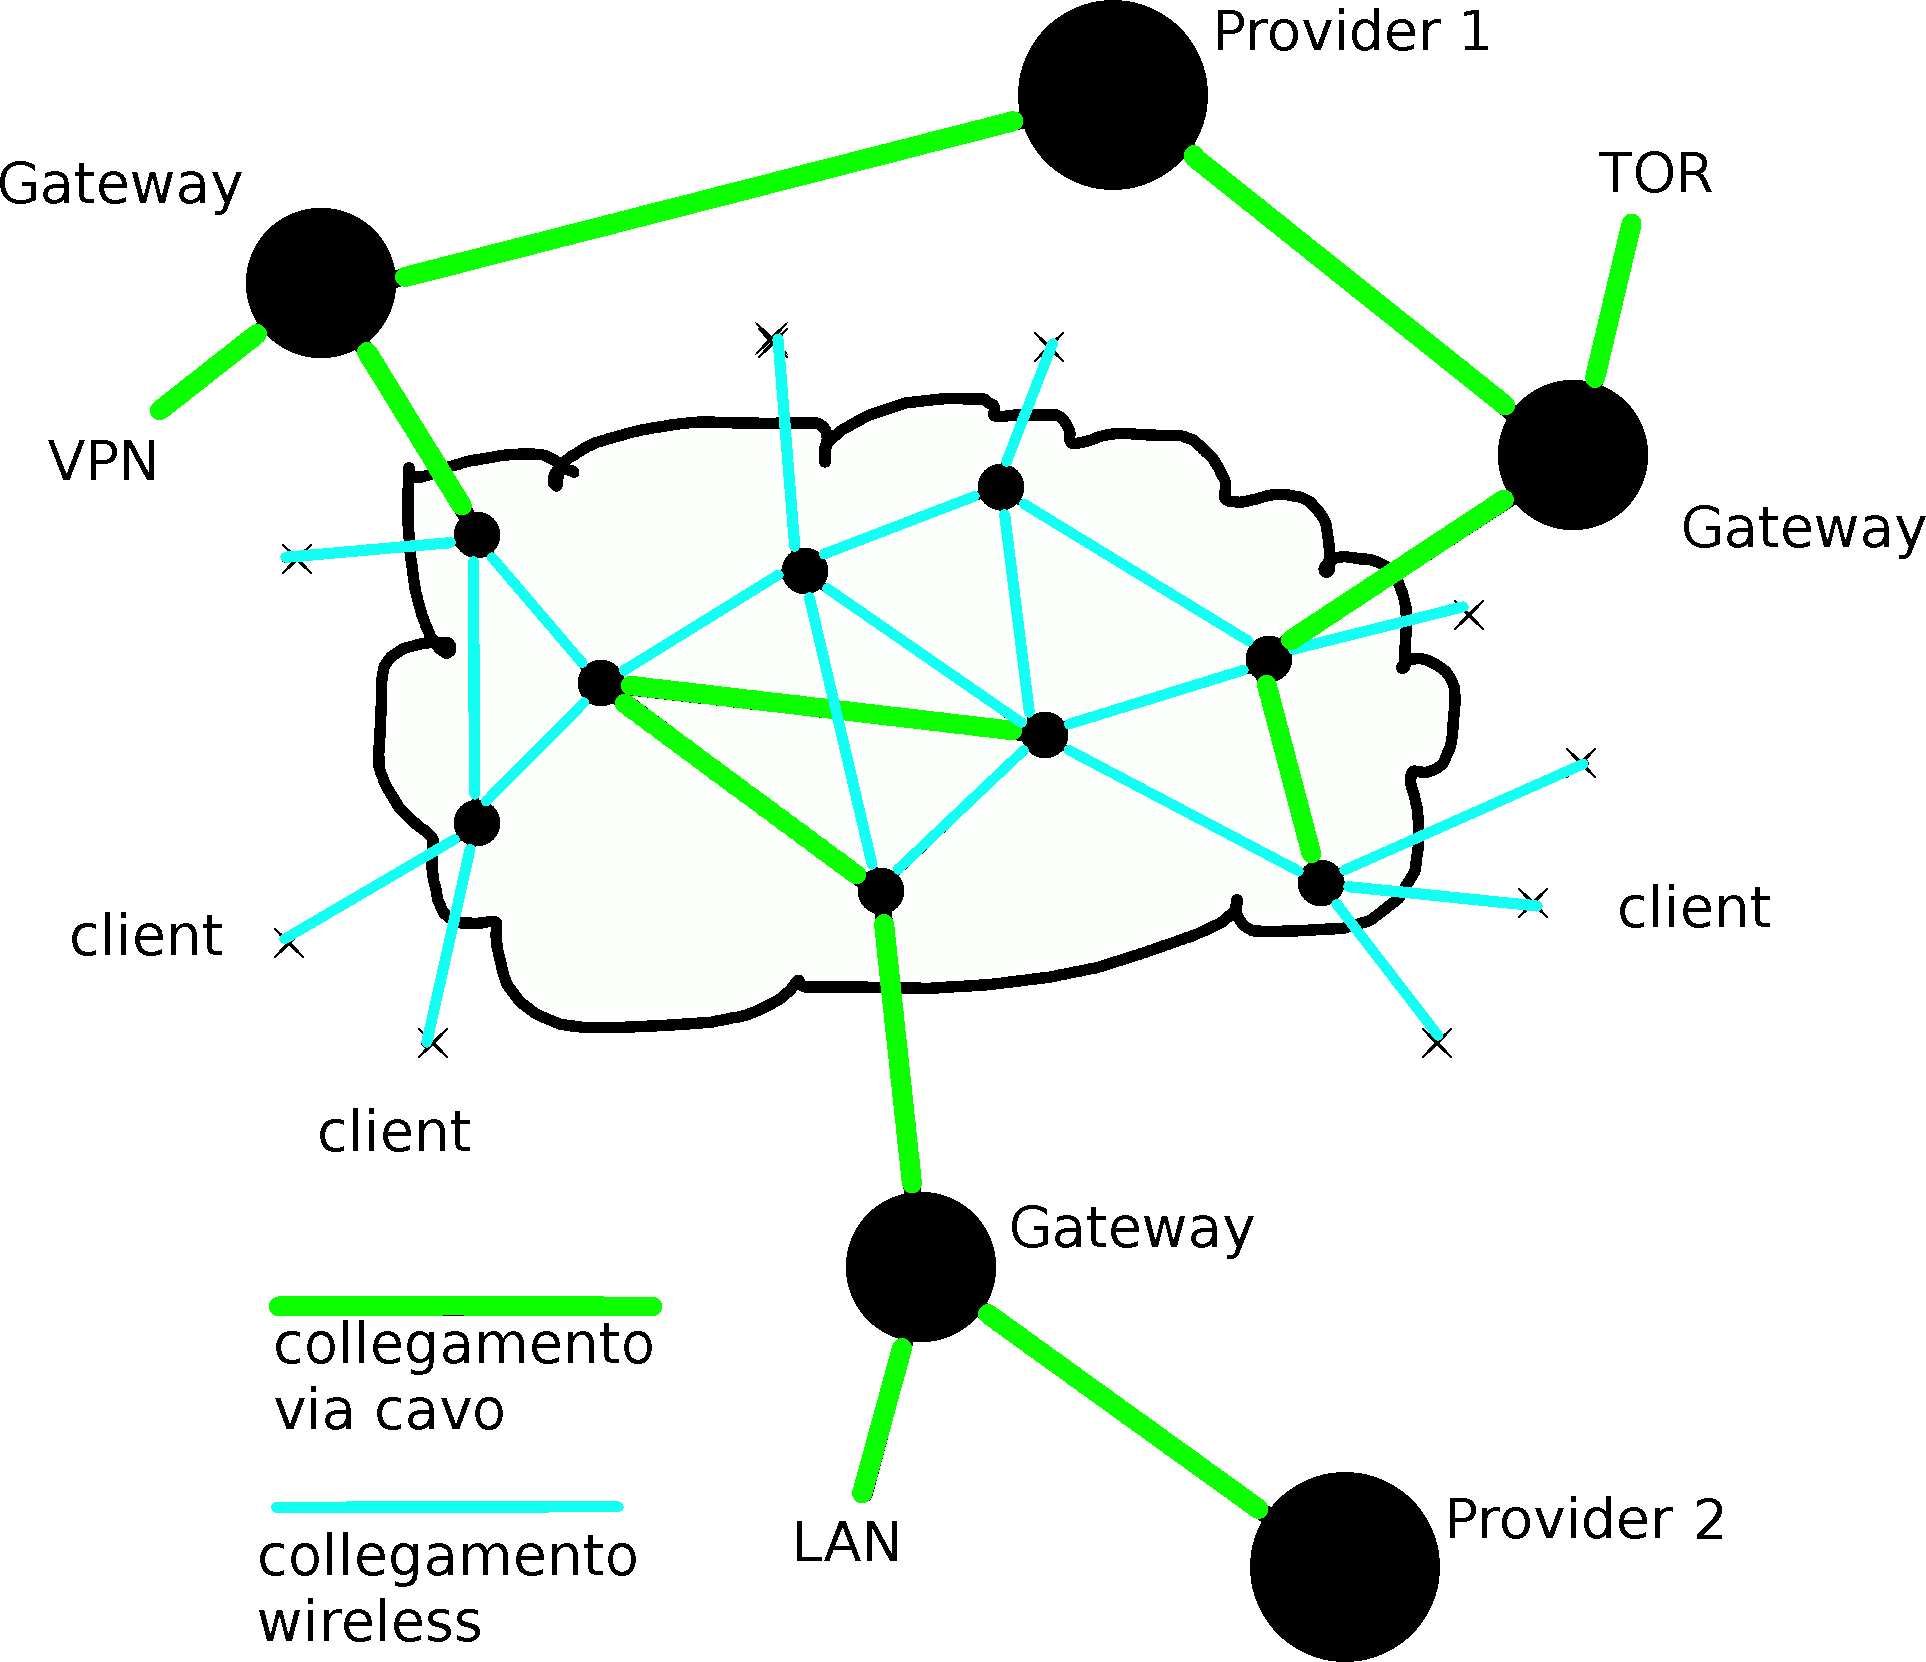
\includegraphics[width=1\textwidth]{images/mesh2-small.png}}}\end{figure}
 
\end{columns}

\end{frame}


\begin{frame}\frametitle{Routing}
Protocolli di routing in EigenNet:
\begin{itemize}
 \item BATMAN-adv, opensource, routing locale, layer 2 (basato sui MAC address).
\pause
\begin{itemize}
 \item La rete si comporta come un grande switch (multicast, auto-configurazione).\pause
 \item Ottimo per reti cittadine (non scala su grandi reti).\pause
 \item Layer 3 agnostic (trasparente per IPv4, IPv6, IPX, $\cdots$).\pause
 \item Roaming dei clients nativo.
\end{itemize}\pause
 \item Babel, opensource, routing tra zone, layer 3 (basato sugli IP). \pause
\begin{itemize}
 \item Protocollo di routing tra comunità ``indipendenti''.\pause
 \item Scala (route aggregation).\pause
 \item Molto configurabile.
\end{itemize}
\end{itemize}

\end{frame}

\subsection{Firmware}
\begin{frame}\frametitle{Firmware}
\textbf{Firmware = OpenWrt + EigenNet}

\vspace{10pt}
OpenWrt:
\begin{itemize}
 \item Distribuzione Linux per embedded.
 \item Estensibile (ha perfino un gestore dei pacchetti!).
\end{itemize}
\pause

EigenNet:
\begin{itemize}
 \item Pacchetto per OpenWrt.\pause
 \item Flash'n'go: configura automaticamente il nodo senza bisogno di un controller centralizzato.\pause
 \item Eventuale customizzazione semplificata.\pause
 \item Crea una rete distribuita senza single point of failure.\pause
 \item Supporto IPv6 nativo.
\end{itemize}

\end{frame}


\begin{frame}\frametitle{Firmware}
Esempio di autoconfigurazione:\\ {\color{blue}abilitare la connessione di clients su una antenna}.
\begin{block}{\textsc{Con Auto-Configurazione}}
\pause
Nel file \texttt{/etc/config/eigennet}

\texttt{option wifi\_clients '{\color{red}true}'}

\end{block}
\end{frame}

\logo{}
{\setbeamertemplate{navigation symbols}{}
\begin{frame}\frametitle{Firmware}
Esempio di autoconfigurazione:\\ {\color{blue}abilitare la connessione di clients su una antenna}.
 \begin{alertblock}{\textsc{Senza Auto-Configurazione}}
\pause
{\small Nel file \texttt{/etc/config/wireless}}

\texttt{\tiny config wifi-iface 'apradio0'\\
\hspace{0.5cm}	option device 'radio0'\\
\hspace{0.5cm}	option network 'clients'\\
\hspace{0.5cm}	option sw\_merge '1'\\
\hspace{0.5cm}	option mode 'ap'\\
\hspace{0.5cm}	option ssid 'eigenNet'\\
\hspace{0.5cm}	option encryption 'none'\\
\hspace{0.5cm}	option maxassoc '20'\\}

{\small Nel file \texttt{/etc/config/network}}

\texttt{\tiny config interface 'clients'\\
\hspace{0.5cm}	option proto 'static'\\
\hspace{0.5cm}	option type 'bridge'\\
\hspace{0.5cm}	list ifname 'bat0'\\
\hspace{0.5cm}	list ifname 'eth0'\\
\hspace{0.5cm}	option ip6addr '2001:1418:1a9:eeab::74EA:3AD6:56A7/64'\\
\hspace{0.5cm}	option ip6gw '2001:1418:1a9:eeab::1000'\\
\hspace{0.5cm}	option ipaddr '192.168.1.21'\\
\hspace{0.5cm}	option netmask '255.255.255.0'\\
\hspace{0.5cm}	option gateway '192.168.1.1'\\}
\end{alertblock}
\end{frame}}

\logo{
\includegraphics[width=0.1\paperwidth]{images/eigenlab-small.png}}
 

\section{Le community wireless nella realtà}

\subsection{Legislazione italiana}
\begin{frame}\frametitle{Legislazione italiana}
L'italia è stato probabilmente il paese Europeo con le leggi più ambigue in materia di Wi-Fi.

\vspace{10pt}
\textbf{Ma il trend è cambiato!}

\begin{itemize}
 \item I collegamenti wifi tra privati sulle frequenze collettive (2.4 GHz, 5 GHz, 17 GHz) sono stati liberalizzati dal nuovo codice delle comunicazioni elettroniche entrato in vigore il 6 giugno 2012.
 \item Condividere la propria connessione WIFI liberamente non è più illegale da quando il decreto Pisanu non è stato prorogato.
\end{itemize}
Altre informazioni: \url{http://wiki.ninux.org/LeggiWireless}
\end{frame}

\logo{}
\subsection{In Italia}
\begin{frame}\frametitle{In Italia}
\begin{columns}
\column{0.6\linewidth}
In Italia stanno nascendo moltissime nuove community wireless.

\vspace{10pt}
Già avviate:
\begin{itemize}
 \item Roma: Ninux Roma (circa 120 nodi!!)
 \item Pisa: EigenNet
 \item Firenze
 \item Viterbo
 \item Calabria (Reggio Calabria, Cosenza, Catanzaro):\\Ninux Calabria
 \item Friuli: Iulii
 \item Sicilia (Mistretta e Vittoria) 
\end{itemize}

\column{0.4\linewidth}
In progetto:\vspace{-10pt}
\begin{figure}{\centering{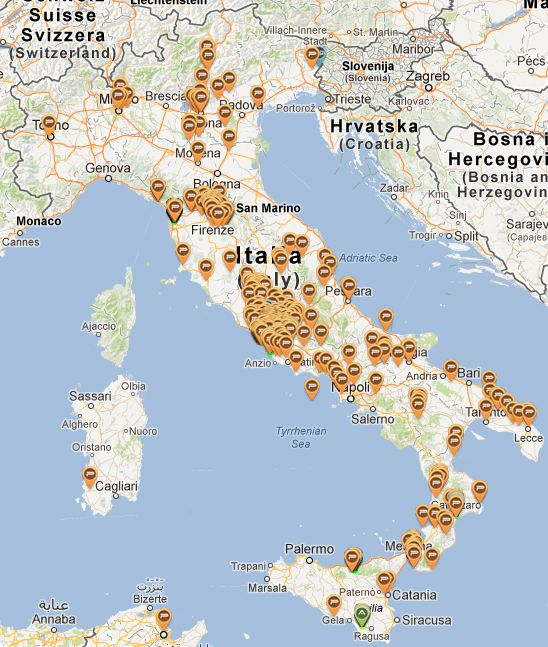
\includegraphics[width=1\textwidth]{images/potenziali-small.jpg}}}\end{figure}
\vspace{-10pt}\hspace{5pt}\textbf{\Large\color{red}Aggiungetevi su\\ \hspace{10pt}\url{map.ninux.org}!}
\end{columns}
\end{frame}


\begin{frame}\frametitle{In Italia}
\begin{columns}
\column{0.4\linewidth}
{\Large Roma}
\begin{figure}{\centering{
\includegraphics[width=1\textwidth]{images/ninux-indicizzato.png}}}\end{figure} 
\column{0.6\linewidth}
\vspace{-15pt}
\begin{figure}{\centering{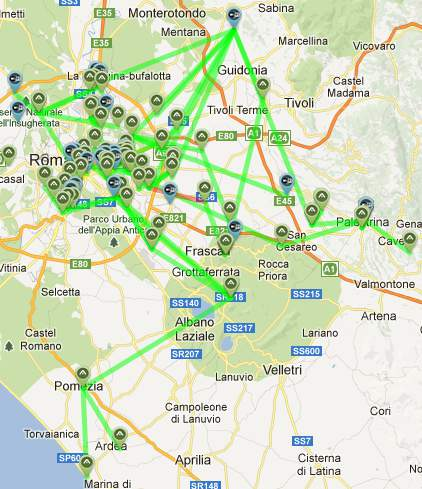
\includegraphics[width=0.95\textwidth]{images/ninux2012-small.jpg}}}\end{figure} 
\end{columns}
\end{frame}

\subsection{Nel Mondo}
\begin{frame}\frametitle{Nel Mondo}
\begin{columns}
\column{0.4\linewidth}
{\Large Grecia}
\begin{figure}{\centering{
\includegraphics[width=1\textwidth]{images/awmn_logo-small.png}}}\end{figure} 
\column{0.6\linewidth}
\begin{figure}{\centering{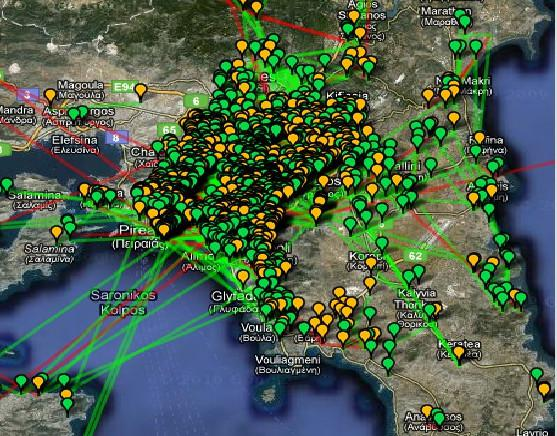
\includegraphics[width=1\textwidth]{images/mapserver-agwm-grecia-small.jpg}}}\end{figure} 
\end{columns}
\end{frame}


\begin{frame}\frametitle{Nel Mondo}
{\Large Catalunia, Spagna}\hspace{10pt}

\includegraphics[width=0.5\textwidth]{images/guifi.png}

\begin{figure}{\centering{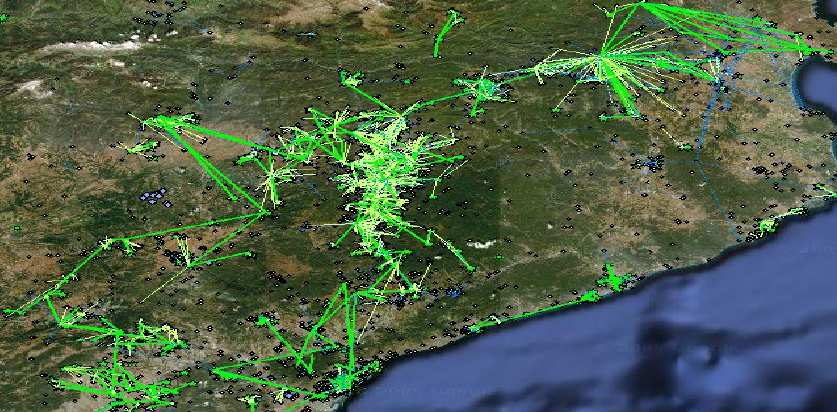
\includegraphics[width=1\textwidth]{images/mapserver-guifi-catalogna-small.jpg}}}\end{figure} 

\end{frame}

\logo{
\includegraphics[width=0.1\paperwidth]{images/eigenlab-small.png}}

\section{}
\begin{frame}

\begin{columns}
\column{0.65\linewidth}

\hspace{1cm}{\Huge{\color{green}Domande?}}\\
\vspace{5pt}
Ulteriori informazioni:\\
\url{www.eigenlab.org}\\
\url{wiki.eigenlab.org}\\
\url{wiki.ninux.org}\\
\textbf{info@eigenlab.org}\\
\textbf{Mailing List}: \url{nnx.me/eigenlab}\\
\textbf{sede di eigenLab} nel giardino tra il Polo Fibonacci e la Sala Studio Pacinotti.
%lunedì 29 ``serata EigenNet'' nella nostra sede\\
%tavolo qui fuori.

\vspace{10pt}
 \small{Si ringraziano per questa presentazione:\\ Ilario Gelmetti (LaTeX, contenuti e scrittura),\\ Federico Capoano (immagini e spunti),\\ David Picconi (template grafico),\\ GULP Pisa (ospitalità e organizzazione!).}\\
\vspace{5pt}
\column{0.4\linewidth}
\begin{figure}{\vspace{-30pt}\centering{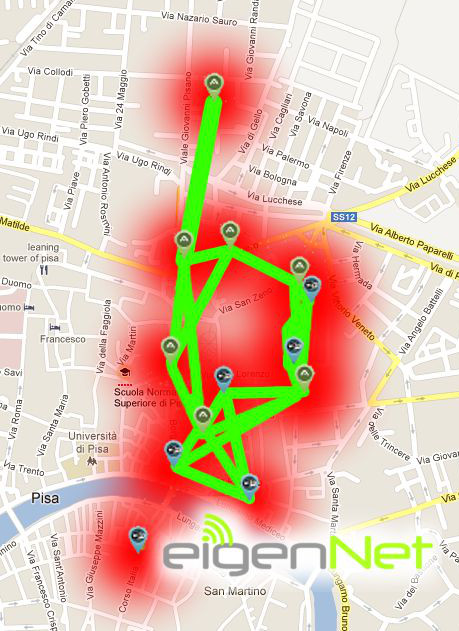
\includegraphics[width=1\textwidth]{images/mappa.jpg}}}\end{figure}
\end{columns}
{\scriptsize{Realizzato da Ilario Gelmetti usando Beamer e \LaTeX}. Licenza CC: BY-NC-SA.}

\end{frame}



\end{document}
